\chapter{Double decker: A memory management framework for derivative clouds}



  \section{Application cache sensitivity}
  
    \subsection{Provisioning of caches at different levels based on application sensitivity}
    
    \subsection{Inability of cache partitioning framework to support anonymous memory applications}
    
    

  \section{Rethink of existing design}
  
    \subsection{Decentralized memory management framework}
	      
      \subsubsection{Native provider cache partitioning framework}

      \subsubsection{Derivative provider memory management framework}	

    \subsection{Hybrid cache}
      
      \subsubsection{Multilevel configurable caches}
      
      \subsubsection{Movement of cache objects}
      
	
  
  \section{Implementation details}
      
    \subsection{Existing implementation status}
    
    \subsection{Hybrid cache}
    
      \subsubsection{Pools to accommodate both memory and SSD objects}
      
      \subsubsection{Asynchronous kernel threads for movement of objects}
      
      \subsubsection{Multilevel stats}
  
  \newpage
  
  \section{Correctness of implementation}
  
    \subsection{Experimental setup}
	
      The following section describes the experimental setup used to verify the correctness of our implementation. 
	
      \myparagraph{Experimental configurations}	
	The set of configurations used for an analysis of memory management framework for a derivative environment must be relevant, and easy to apply. The following configurations
fit this criteria, and have been used for the evaluation.

	  \begin{itemize}
	   \item \textbf{Memory Requirement:} Memory requirement of each container, the estimated total memory used by a container.
	   
	   \item \textbf{Container memory limit:} Size of memory allocated to a container at the Cgroup level (soft and hard limits). 
	   \item \textbf{Memory cache limit:} Size of memory (L1) cache assigned to a container. 
	   \item \textbf{SSD cache limit:} Size of SSD (L2) cache assigned to a container.
	   
	   \item \textbf{Workload:} Workload application that is running inside each of the container. 
	   \item \textbf{Number of containers:} Number of containers that are currently executing in the system.
	   \item \textbf{Number of VMs:} Number of virtual machines that are currently executing in the system.
	  \end{itemize}	  
	  
	  For the sake of simplicity in the evaluations of correctness of our setup. We have only considered a single container, single VM setup 
	  which makes use of synthetic workload to stress our system.
	
      \myparagraph{Metrics of interest}	
	The following are the metrics of interest that would help us establish the correctness of our implementation.
	  
	  \begin{itemize}
	   
	   \item \textbf{Container memory usage:} Guest memory usage of the container.
	   \item \textbf{Memory cache usage:} Memory cache used by the container.
	   \item \textbf{SSD cache usage:} SSD cache used by the container.
	   
	   \item \textbf{Demoted:} Objects moved from memory to SSD cache.
	   \item \textbf{Promoted:} Objects moved from SSD to memory cache.
	   
	  \end{itemize}	  
	  
	  The following metrics are collected both for memory and SSD cache
	  
	  \begin{itemize}
	   
	   \item \textbf{Puts:} Number of objects successfully put into this container cache.
	   \item \textbf{Gets:} Number of objects successfully got from this container cache.
	   \item \textbf{Flushes:} Number of objects flushed from this container cache.
	   \item \textbf{Evicts:} Number of objects evicted from this container cache.
	   
	  \end{itemize}	  
	  
	
      \myparagraph{Workload}	
	For establishing the correctness of our workload, we have considered a self generated workload generated using \texttt{cat} command 
	that outputs the content of a file onto \texttt{/dev/null}.
	
      \myparagraph{Testbed}
	Our testbed consists of a single VM, single container running on top of our hybrid implementation of Double decker as shown 
	in Fig~\ref{img_correctness_testbed}. The hypervisor used is KVM, and the container manager used is LXC.  
	
	
	\noindent The physical machine configuration used is as described below,
	  \begin{enumerate}
	   \item Intel(R) Core(TM) i7-3770 CPU @ 3.40GHz
	   \item 4 CPU cores (with multi-threading)
	   \item 8 GB of physical RAM
	   \item 120 GB SSD disk
	  \end{enumerate}

	
	\begin{figure}
	  \centering
	  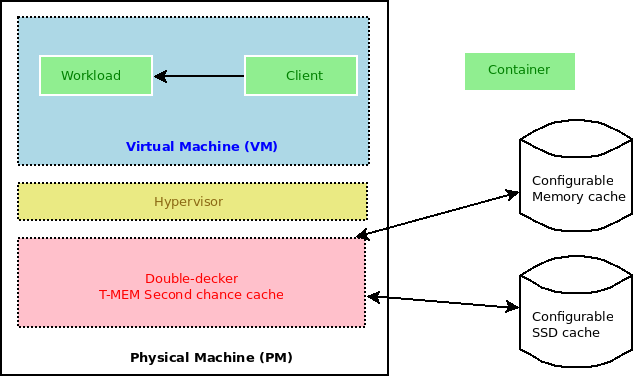
\includegraphics[width=0.9\textwidth]{images/correctness/exp_setup.png}
	  \caption{Experimental testbed for checking correctness}
	  \label{img_correctness_testbed}
	\end{figure}
  
    \subsection{Arithematic validation of stats}
    
    \subsection{Movement of objects between both levels of cache}
	
	\subsubsection{Memory to SSD cache}

	  \myparagraph{Question}
	    To verify the correctness in accounting of stats while accessing cache and moving objects from memory (L1) to SSD (L2) cache.
	    
	  \myparagraph{Procedure}
	    H
	
	\subsubsection{SSD to memory cache}
    
  
  
  
  \section{Evaluation of Double Decker}
  
    \subsection{Experimental setup}
	
	\paragraph{Experimental configurations}
	
	\paragraph{Metrics of interest}
	
	\paragraph{Workload}
	
	\paragraph{Testbed}
  
    \subsection{Provisioning for anonymous and file backed workloads}
    
    \subsection{Hybrid cache provisioning}
    